\documentclass{article}

%%%%%%%%%%%%%%%%%%%%%%%% Importation de paquets %%%%%%%%%%%%%%%%%%%%
\usepackage{polyglossia}
\usepackage{graphics}
\usepackage{fontspec}
\usepackage{fancyhdr}
\usepackage{listings}
\usepackage{graphics}
\usepackage{fancyhdr}
\usepackage{vmargin}
\usepackage{epsfig}   
\usepackage{multicol}
\usepackage{multirow}

%%%%%%%%%%%%%%%%%%%%%%%% Format, langue, marges %%%%%%%%%%%%%%%%%%%%%%%%%%

\setdefaultlanguage{english}
\defaultfontfeatures{Mapping=tex-text,Scale=MatchLowercase}
\setmainfont{Linux Libertine O}
\setpapersize{A4}
\setmarginsrb   
{35mm}  % leftmargin
{20mm}  % topmargin
{35mm}  % rightmargin
{40mm}  % bottommargin
{14pt}  % headheight
{15mm}   % headsep
{20pt}  % footheight
{20mm}  % footskip

%%%%%%%%%%%%%%%%%%%%%%%% En-tete et pied de page %%%%%%%%%%%%%%%%%%%%%%%%%%
\pagestyle{fancy}
\fancyhf{}
\lhead{\scalebox{0.1}[0.1]{
\includegraphics{./Images/enseeiht}}}
\rhead{\scalebox{0.1}[0.1]{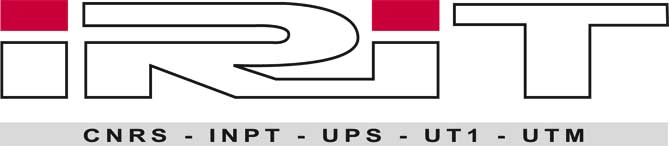
\includegraphics{./Images/irit}}
\lfoot{Three-dimensional modeling and printing}}
\rfoot{\bfseries \thepage}

\begin{document}

\bigskip
\bigskip
\bigskip
\bigskip
\bigskip
\bigskip
\bigskip
\bigskip

\begin{center}
\LARGE{Three-dimensional modelling and printing project :\\User documentation \\}
\bigskip
\bigskip\begin{tiny}
\end{tiny}
\Large{from January 23 to March 16, 2012}
\end{center}

\bigskip
\bigskip

\begin{center}
\large{
\textit{Vincent \textsc{Duvert} \\
Antoine \textsc{Lubineau} \\
Caroline \textsc{Naud} \\
James \textsc{Packer} \\
Florian \textsc{Ribon}} \\
\bigskip
INP-ENSEEIHT/IMA 
}
\end{center}

\bigskip
\bigskip

	This report summarizes the context, organization, work and outcomes within the project 3D modeling and printing project suggested by the VORTEX team of IRIT to some of the third-year students in the IMA department of ENSEEIHT.

\bigskip
\bigskip

\begin{figure}[!h]
\begin{center}
\scalebox{0.4}[0.4]{
\includegraphics{./Images/enseeiht}}
\end{center}
\end{figure}

\bigskip

\begin{center}
http://www.enseeiht.fr/fr/index.html \\
2 Rue Charles Camichel \\
31 071 TOULOUSE
\end{center}

\bigskip

\begin{figure}[!h]
\begin{center}
\scalebox{0.4}[0.4]{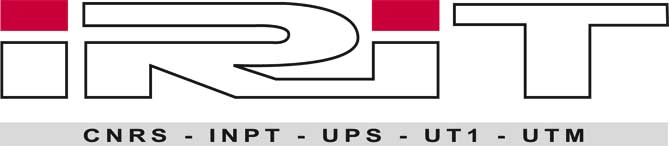
\includegraphics{./Images/irit}}
\end{center}
\end{figure}

\begin{center}
http://www.info@irit.fr\\
Université Paul Sabatier \\
118 Route de Narbonne \\
F-31062 TOULOUSE CEDEX 9
\end{center}

\thispagestyle{empty}

\newpage

\tableofcontents

\newpage

\section{Reminding of the global architecture of the application}


\begin{figure}[!h]
\begin{center}
\scalebox{0.4}[0.4]{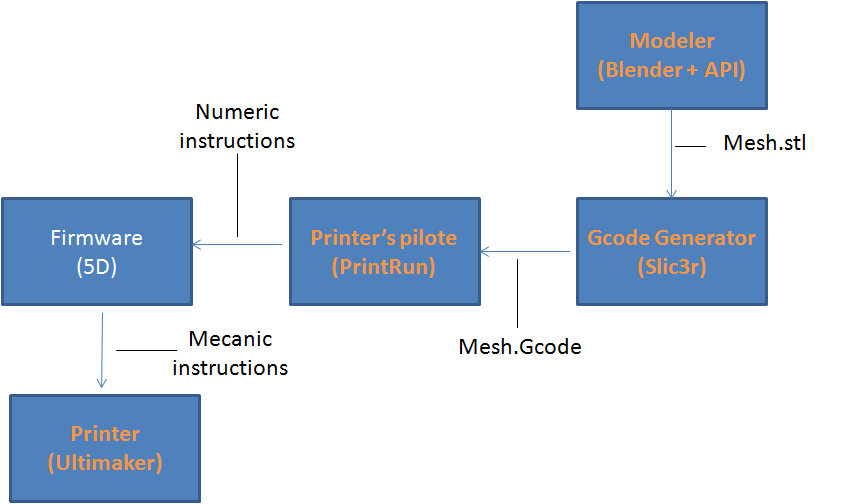
\includegraphics{./Images/ARD1}}
\end{center}
\end{figure}

\newpage

\section{The modelling part on Blender}

\subsection{Point on the graphic interface}

Mettre des Imprim écrans

\subsection{Obtaining a mesh}

\subsubsection{Loading a mesh for your personnal files}

\subsubsection{Editing your own mesh}

\subsection{Verifying the quality of your mesh}

\subsection{Generating adequate supporting plans for your object}

\subsection{Choosing a good supporting plan}

\subsection{Saving your mesh}

\newpage

\section{The printing part}

\subsection{Preparing the Utimaker 3D printer}

\subsection{Generating the GCode on Slic3r}

\subsection{Sending the instructions to the printer with PrintRun}

\newpage

\section{Ending the work}

Comment fermer toutes les application après avoir sauvé une configuration \\
Parler de polir l'objet \\

\end{document}
